\subsection{Extended Kalman Filter} \label{ssec:framework_ekf}
% Kalman Filter
The Kalman Filter (KF) is a useful algorithm to analyze a dynamical system that can be modeled regardless of how uncertain the information that is known about it is~\cite{rauch1965maximum}.
Its utility is given by the fact that it can estimate the current state of a process while minimizing the average quadratic error (described in Appendix \ref{add:errors}) using only the measurement system and the last state, without requiring access to the whole chain of events previous to the current one~\cite{einicke2006optimal}.
Kalman filters are commonly used for control of vehicles, signal processing and econometrics~\cite{zarchan2013fundamentals}.

This filter, also known as the Linear Quadratic Estimator (LQE), is an algorithm that estimates the value and uncertainty of variables associated to a statistical noise using a series of measurements through time~\cite{kalman1960new}, representing the variables as a state vector $\mathbf{x}_k$ and an observation (or measurement) vector $\mathbf{z}_k$ for an arbitrary moment on time or ``timestep'' denominated $k$.

% Extended Kalman Filter
The basic Kalman Filter, as useful as it is, is limited in the sense that it assumes that the model is linear, and thus is of little use when facing problems with non-linear processes or observation models~\cite{simon2006optimal}.
For this type of problems, the so-called Extended Kalman Filter (EKF) is used~\cite{karimipour2015extended}, which only requires the functions used to predict the next state and the next observation to be differentiable.
It linealizes over an estimation of the current expected value and the covariance of the state vector.
It's worth noting that the cited textbook explains the original work from $1959-1961$ since no publications were found explaining the EKF from that time by the author.

Different from its linear counterpart, the EKF is not an optimum estimator, and if fed an erroneous initial vector it can quickly diverge.
The estimated covariance matrix can also underestimate the real covariance matrix, being sometimes inconsistent without the addition of stabilization noise~\cite{julier1997new}.
Due to this and the sometimes inefficient calculation of Jacobian matrices (described in addendum \ref{add:jacobian_matrix}) necessary for the EKF, it is often preferred to use the Unscented Kalman Filter (UKF)~\cite{julier1997new}.

Regardless, for the specific case of CLAS12, it was decided during development that only the EKF was necessary since, as described in Section \ref{ssec:framework_dc}, the filter is fed preprocessed data with already some degree of precision.
While not linear, the \textbf{predict} and \textbf{update} functions (explicitly defined in Section \ref{ssec:framework_tf}), are quasi-linear and their Jacobian matrices aren't complicated enough as to require the usage of the UKF, with them only being $5\times5$.
% Note: This could use a citation but it came from a conversation with Veronique so idk.

\newpage

To describe the Extended Kalman Filter (EKF) and derive its computational complexity, it is necessary first to provide a mathematical formulation for the next state $\mathbf{x}_k$ and the obtained measurements $\mathbf{z}_k$ with transition functions $\mathbf{f}(\mathbf{x}, \mathbf{u})$ and $\mathbf{h}(\mathbf{x})$ respectively:
    \begin{align*}
        \mathbf{x}_k &= \mathbf{f}(\mathbf{x}_{k-1}, \,\mathbf{u}_k) + \mathbf{w}_k\\
        \mathbf{z}_k &= \mathbf{h}(\mathbf{x}_k) + \mathbf{v}_k\,.
    \end{align*}
    
% \newpage

    \begin{figure}[ht]
        \centering
        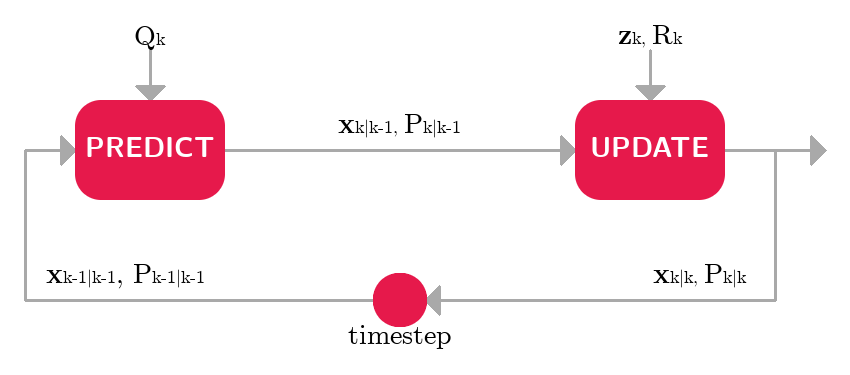
\includegraphics[scale=0.50]{ekf_diagram}
        \caption{\label{fig:ekf_diagram} System diagram showing the EKF process to estimate a state vector $\mathbf{x}_{k|k}$ and its covariance matrix $P_{k|k}$ from $\mathbf{x}_{k-1|k-1}$, $P_{k-1|k-1}$ and $\mathbf{z}_k$ with noise matrices $Q_k$ and $R_k$.}
    \end{figure}
    
where $\mathbf{u}_k$ is the control vector and $\mathbf{w}_k$ and $\mathbf{v}_k$ are the errors in the measurement process, which are assumed to be Gaussian noises with an average of zero and with covariance matrices $Q_k$ and $R_k$ respectively.
For the purposes of this project the control vector $\mathbf{u}_k$ is left as $\mathbf{0}$ considered that it denotes user input, which isn't present in this model.

A note on the notation: $k_1|k_2$ refers to state in step $k_1$ given the information known in step $k_2$, where $k_1$ and $k_2$ are arbitrary steps.
Based on this, $\mathbf{x}_{k|k-1}$ is the state vector $\mathbf{x}$ in step $k$ knowing the information from $k-1$.
The exact logic on how this is updated is related to the measurement vector and is explained later in this section.

The transition and observation matrices $J_{\mathbf{f}(k)}$ and $J_{\mathbf{h}(k)}$ are also defined as the following Jacobian matrices:
    \begin{align*}
        J_{\mathbf{f}(k)} &= \frac{\partial \mathbf{f}}{\partial \mathbf{x}}\Bigr|_{\substack{\mathbf{\hat{x}}_{k-1|k-1}}}\\
        J_{\mathbf{h}(k)} &= \frac{\partial \mathbf{h}}{\partial \mathbf{z}}\Bigr|_{\substack{\mathbf{z}_{k}}}\,.
    \end{align*}

\newpage

To calculate the computational complexity of the algorithm, the size of the state vector $\mathbf{x}_k$ is first defined as $n$ and the size of the measurement vector $\mathbf{z}_k$ as $m$, while also defining the computational cost of applying the functions $\mathbf{f(\mathbf{x}, \mathbf{u})}$ and $\mathbf{h}(\mathbf{x})$ on an arbitrary input as $\text{C}(\mathbf{f}(\cdot,\cdot))$ and $\text{C}(\mathbf{h}(\cdot))$ respectively.

% \newpage

To obtain the next state two steps are required, \textbf{Predict} and \textbf{Update}.
The former requires the following computations to obtain the estimate $\mathbf{\hat{x}}_{k|k-1}$ and the covariance matrix $P_{k|k-1}$ \textit{a priori}:
    \begin{align*}
        \mathbf{\hat{x}}_{k|k-1} &= \mathbf{f}(\mathbf{\hat{x}}_{k-1|k-1}, \mathbf{u}_k) &\rightarrow \text{C}(\mathbf{f}(\cdot, \cdot))\\
        P_{k|k-1} &= J_{\mathbf{f}(k)} P_{k-1|k-1} J_{\mathbf{f}(k)}^T + Q_k &\rightarrow 2n^3 + n^2\,,
    \end{align*}

Then, to calculate the estimated state $\mathbf{\hat{x}}_{k|k}$ and the covariance matrix $P_{k|k}$ \textit{a posteriori}, the following calculations are done in the latter step:
    \begin{align}
        \nonumber &\mathbf{\tilde{y}}_k = \mathbf{z}_k - \mathbf{h}(\mathbf{\hat{x}}_{k|k-1}) &\rightarrow m + \text{C}(\mathbf{h}(\cdot))\\
        &S_k = J_{\mathbf{h}(k)} P_{k|k-1} J_{\mathbf{h}(k)}^T + R_k &\rightarrow n^2m + nm^2 + m^2 \label{eq:ekf_Sk}\\
        &K_k = P_{k|k-1} J_{\mathbf{h}(k)}^T S_k^{-1} &\rightarrow n^2m + nm^2\label{eq:ekf_Kk}\\
        \nonumber &\mathbf{\hat{x}}_{k|k} = \mathbf{\hat{x}}_{k|k-1} + K_k \mathbf{\tilde{y}}_k &\rightarrow nm + m\\
        &P_{k|k} = (I - K_k J_{\mathbf{h}(k)}) P_{k|k-1} &\rightarrow n^2m + n^2\,,\label{eq:ekf_Pk}
    \end{align}
where $\mathbf{\tilde{y}}_k$ is the called residual measurement of the step $k$, $S_k$ is its covariance matrix, named residual covariance matrix, and $K_k$ is defined as the Kalman gain during that step.
The Kalman gain is a matrix of gain from each measurement to each estimation, and if it's zero then $\mathbf{x}_{k|k} = \mathbf{x}_{k|k-1}$.

To calculate the computational complexity of each step, it is assumed that the complexity of multiplying two matrices of the same size $p\times p$ is $O(p^3)$, multiplying matrices of sizes $p\times q$ and $q\times r$ is $O(p\,q\,r)$ and inverting a matrix of size $p\times p$ has a complexity of $O(p^3)$.
Considering that the computation of $P_{k|k-1} (J_h)_k^T$ in step \eqref{eq:ekf_Sk} is reused in step \eqref{eq:ekf_Kk}, the total complexity at an arbitrary step $k$ of the algorithm is the following:
    \begin{align*}
        \text{C}(\mathbf{f}(\cdot, \cdot)) + \text{C}(\mathbf{h}(\cdot)) + 2n^3 + 2n^2(1+m) \\+ n(1+m+2m^2) + m(1+m)\,,
    \end{align*}
and in Big O notation:
    \begin{align}
        \text{O}(\text{C}(\mathbf{f}(\cdot, \cdot)) + \text{C}(\mathbf{h}(\cdot)) + n^3 + n^2m + nm^2)\,.
    \end{align}